\section{SEAL library}

The SEAL library is a C++, open source cryptographic software library, developed by Microsoft. It's the tool we used in our project to codify, encrypt, decrypt and decodify the data to be manipulated. We also used the library for the activation function layers in the neural network. In this section we will show in detail the wrapper we created to invoke the SEAL functions from python.

\subsection{The encrypted polynomials ring}

As we have already mentioned in the cryptography section, SEAL does not directly implement the FV scheme, but instead makes some changes to this homeomorphic algorithm. In particular, as we have already seen, the Chinese remainder theorem is used to break down the parameter $q$ into various divisors $q_i$, all with a maximum of 60 bits. Moreover, an encrypted message is not an array of polynomials in $R^n_q$, is actually an array of polynomials in $R^{n+1}_q$. It is important to keep this point in mind while programming the operations: for example, the polynomial-scalar sum must be performed once every $n+1$ coefficients, for each $q_i$ of the first size. An encrypted message, in fact, is formed as follows:

\begin{figure}[H]
	\centering
	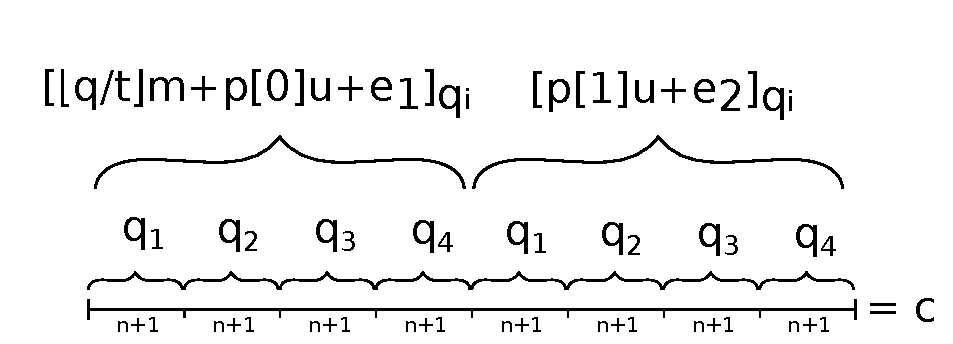
\includegraphics[width=\textwidth]{images/fig3.pdf}
    \caption{The encrypted message scheme.}
    \label{fig:im3}
\end{figure}

In this example we have a module $q$ composed of four divisors ($q1$, $q2$, $q3$, $q4$), and the encrypted message has size equal to 2. Therefore we have a total of 8 polynomials, and each polynomial has degree $n$, for a total of $(n+1)\cdot8$ coefficients. This is the minimum number of coefficients needed to encode $n$ values of the input data. Of the 8 polynomials, the first four contain the original information $(\lfloor q/t \rfloor m)$, the other four contain instead only information on the added noise, so that, together with the secret key, the message can be decrypted. The coefficients of the eight polynomials are reduced modulo $q_i$, with $i$ based on the position of the polynomial. In particular they are repeated: $i = 1,2,3,4$ for the first half, and again $i = 1,2,3,4$ for the second half. All this must be taken into account when programming the neural network. (see the Section 3: Neural network).

\subsection{The wrapper}

The wrapper for the SEAL library consists of two parts: a \texttt{wrapper.cpp} file and a \texttt{wrapper.py} file. We first introduce the C++ part, and then we'll show the Python part.

\subsubsection{The C++ wrapper}

The \texttt{wrapper.cpp} file declares all the functions that must be used in the project. They are:


\lstset{frame=tb,
  language=C++,
  breaklines=true,
  showstringspaces=false,
  columns=flexible,
  numbers=none,
  commentstyle=\color{dkgreen},
  stringstyle=\color{mauve},
  tabsize=3,
  morekeywords={uint64_t}
}
\begin{lstlisting}[frame=single]
void generate_new_keys()
void initialize()
void deallocate()
void encrypt_tensor(uint64_t *input, uint64_t *output, int input_axis0_size, int data_size)
void decrypt_tensor(uint64_t *input, uint64_t *output, int output_axis0_size, int data_size)
void square_tensor(uint64_t *input, uint64_t *output, int input_axis0_size, int data_size)
\end{lstlisting}

The first function generate a new set of keys for the encryption system, and save them in the folder "keys". The initialize() function loads the those keys in memory to be used; the deallocate() function does the opposite, that is, it frees the memory used by the keys and the SEAL library. The three following functions correspond to the three basic operations of encrypting, decrypting and squaring. The important thing to note here is that they take as input an entire tensor, which, in the case of decrypt_tensor($\cdot$) and square_tensor($\cdot$), is a set of encrypted polynomials. encrypt_tensor($\cdot$) instead takes as input a data tensor and converts it into an encrypted polynomial tensor, ie it deals with both CRT batching and actual encryption. Similarly, decrypt_tensor($\cdot$), after decrypting the polynomial tensor, decodes it. The exact number of messages encrypted in output to the encrypt_tensor function depends on the number of images we want to transform, namely input_axis0_size, and the size of each image: data_size. A polynomial of $n$ coefficients can encode up to $n$ values of different images, therefore the number of messages encrypted in output to the function is equal to $\lceil \text{input_axis0_size}/n\rceil\cdot\text{data_size}\cdot5$, where 5 is the number of factors $t_i$ of the $t$ chosen.

\subsubsection{The Python wrapper}

The python part of the wrapper uses ctypes, the Python module, to call the dynamic library compiled by the \texttt{wrapper.cpp} file. It takes care of adapting the data in the useful form to the library in C ++. For example, it takes care of flattening the tensors before passing them as parameters to the function to call, or it calculates the data_size parameter. It has two special methods, __init__() and __del__(), of which the first deals with loading all the necessary data into memory, such as the parameters $n$, $t$, $q$, $k$, and the dynamic library libseal.so, and the second deallocates the library from the ram, freeing the memory from previously loaded data.

\subsection{The selected parameters for the cryptography scheme}

As discussed above, one of the differences between the SEAL version used in \cite{dowlin2016cryptonets} and the one that we use is the need, in our case, to break down the parameter $q$ into several divisors. This prevents us from using the same identical parameters used by that paper, since the numbers chosen for the parameter $q$ in the original project are prime numbers. We have therefore decided to keep the choices of the other two parameters ($n$ and $t$) identical and to change only $q$. It is important to note that, due to the decomposition of the $t$ parameter, these parameters are not part of a single encryption scheme, but rather there are 5 schemes: one for each $t_i$. So for each $t_i$ we decided to keep the number of coefficients $n$ (as in \cite{dowlin2016cryptonets}), and the parameters $q$ (differently from how it was done in the original project). Therefore, the five schemes are:

\begin{center}
\begin{tabular}{ |c|P{2cm}|P{2cm}|c| } 
\hline
Scheme number & n & t & q \\
\hline
\hline
& & & \\
\multirow{4}{*}{\#1} & \multirow{4}{*}{4096} & \multirow{4}{*}{40961} & 36028797014376449 \\
& & & 36028797013327873 \\
& & & 1152921504241942529 \\
& & & 1152921504369344513 \\
& & & \\
\hline
& & & \\
\multirow{4}{*}{\#2} & \multirow{4}{*}{4096} & \multirow{4}{*}{65537} & 36028797014376449 \\ 
& & & 36028797013327873 \\ 
& & & 1152921504241942529 \\ 
& & & 1152921504369344513 \\ 
& & & \\
\hline
& & & \\
\multirow{4}{*}{\#3} & \multirow{4}{*}{4096} & \multirow{4}{*}{114689} & 36028797014376449 \\ 
& & & 36028797013327873 \\ 
& & & 1152921504241942529 \\ 
& & & 1152921504369344513 \\ 
& & & \\
\hline
& & & \\
\multirow{4}{*}{\#4} & \multirow{4}{*}{4096} & \multirow{4}{*}{147457} & 36028797014376449 \\ 
& & & 36028797013327873 \\ 
& & & 1152921504241942529 \\ 
& & & 1152921504369344513 \\ 
& & & \\
\hline
& & & \\
\multirow{4}{*}{\#5} & \multirow{4}{*}{4096} & \multirow{4}{*}{188417} & 36028797014376449 \\ 
& & & 36028797013327873 \\ 
& & & 1152921504241942529 \\ 
& & & 1152921504369344513 \\ 
& & & \\
\hline
\end{tabular}
\end{center}

Note that for every $i=1,2,3,4,5$, $t_i$ is a prime number and it's equal to 1 (mod $2n$), as required by CRT batching (see the Section 2.3: Chinese remainder theorem). For each combination of $t_i$ and $q_j$ the parameter $k_{ij} = (\lfloor q/t_i \rfloor) \text{ mod } q_j$ is then calculated, necessary for the plain sum, as described above. You can check the parameters in the code inside the \texttt{wrapper.py} file.


